\documentclass[11pt,compress,t,notes=noshow]{beamer}\usepackage[]{graphicx}\usepackage[]{color}

\makeatletter
\def\maxwidth{ %
  \ifdim\Gin@nat@width>\linewidth
    \linewidth
  \else
    \Gin@nat@width
  \fi
}
\makeatother

\definecolor{fgcolor}{rgb}{0.345, 0.345, 0.345}
\newcommand{\hlnum}[1]{\textcolor[rgb]{0.686,0.059,0.569}{#1}}%
\newcommand{\hlstr}[1]{\textcolor[rgb]{0.192,0.494,0.8}{#1}}%
\newcommand{\hlcom}[1]{\textcolor[rgb]{0.678,0.584,0.686}{\textit{#1}}}%
\newcommand{\hlopt}[1]{\textcolor[rgb]{0,0,0}{#1}}%
\newcommand{\hlstd}[1]{\textcolor[rgb]{0.345,0.345,0.345}{#1}}%
\newcommand{\hlkwa}[1]{\textcolor[rgb]{0.161,0.373,0.58}{\textbf{#1}}}%
\newcommand{\hlkwb}[1]{\textcolor[rgb]{0.69,0.353,0.396}{#1}}%
\newcommand{\hlkwc}[1]{\textcolor[rgb]{0.333,0.667,0.333}{#1}}%
\newcommand{\hlkwd}[1]{\textcolor[rgb]{0.737,0.353,0.396}{\textbf{#1}}}%
\let\hlipl\hlkwb

\usepackage{framed}
\makeatletter
\newenvironment{kframe}{%
 \def\at@end@of@kframe{}%
 \ifinner\ifhmode%
  \def\at@end@of@kframe{\end{minipage}}%
  \begin{minipage}{\columnwidth}%
 \fi\fi%
 \def\FrameCommand##1{\hskip\@totalleftmargin \hskip-\fboxsep
 \colorbox{shadecolor}{##1}\hskip-\fboxsep
     \hskip-\linewidth \hskip-\@totalleftmargin \hskip\columnwidth}%
 \MakeFramed {\advance\hsize-\width
   \@totalleftmargin\z@ \linewidth\hsize
   \@setminipage}}%
 {\par\unskip\endMakeFramed%
 \at@end@of@kframe}
\makeatother

\definecolor{shadecolor}{rgb}{.97, .97, .97}
\definecolor{messagecolor}{rgb}{0, 0, 0}
\definecolor{warningcolor}{rgb}{1, 0, 1}
\definecolor{errorcolor}{rgb}{1, 0, 0}
\definecolor{code}{rgb}{0.97, 0.96, 1.0}
\newenvironment{knitrout}{}{} % an empty environment to be redefined in TeX

\usepackage{alltt}
\usepackage[utf8]{inputenc}
\usepackage[ngerman]{babel}
\usepackage{dsfont}
\usepackage{verbatim}
\usepackage{amsmath}
\usepackage{amsfonts}
\usepackage{mathtools}
\usepackage{csquotes}
\usepackage{cmbright}
\usepackage{multirow}
\usepackage{longtable}
\usepackage{enumerate}
\usepackage[absolute,overlay]{textpos}
\usepackage{psfrag}
\usepackage{algorithm}
\usepackage{algpseudocode}
\usepackage{eqnarray}
\usepackage{bytefield}
\usepackage{animate}
\usepackage{tikz}
\usetikzlibrary{shapes,matrix,positioning,chains,arrows,shadows,decorations.pathmorphing,fit,backgrounds}
\usepackage{adjustbox}
\usepackage{colortbl}
\usepackage{tabularx} % for tables (incl. \hline)
\usepackage{arydshln} % Load after array, longtable, colortab and/or colortbl , otherwise problems with \hline in tabular env
\usepackage{etex} %increase registers for \dimenS to more than 256, otherwise we get "No room for a new \dimen"
\usepackage{graphicx}
\usepackage{booktabs} %used in epr lectures
\usepackage{bm} % bold greek letters
\usepackage{hyperref} % url citing
\usepackage{blkarray} % block arrays
\usepackage{listings} % block of code
\usepackage{xcolor} %colored math symbols
\usepackage{pgffor}
\usepackage{verbatimbox}
\usepackage{xcolor}

%some colors
\definecolor{checkgreen}{HTML}{18A126}
\definecolor{errorred}{HTML}{FF0000}
\definecolor{blockbg}{HTML}{F7F7F7}
\definecolor{gray}{HTML}{A0A0A0}

% basic latex stuff
\newcommand{\col}{\par\colorbox{code}{\parbox{\textwidth}{\theverbbox}}\par}
\newcommand{\eg}{e.\,g.\xspace} %for example
\newcommand{\ie}{i.\,e.\xspace} %that is to say...
\newcommand{\pkg}[1]{{\fontseries{b}\selectfont #1}} %fontstyle for R packages
\newcommand{\lz}{\vspace{0.5cm}} %vertical space
\newcommand{\oneliner}[1] % Oneliner for important statements
{\begin{block}{}\begin{center}\begin{Large}#1\end{Large}\end{center}\end{block}}
\def\SpAr{\quad \Rightarrow \quad}

%new environments
\newenvironment{vbframe}  %frame with breaks and verbatim
{
 \begin{frame}[containsverbatim,allowframebreaks]
}
{
\end{frame}
}

\newenvironment{vframe}  %frame with verbatim without breaks (to avoid numbering one slided frames)
{
 \begin{frame}[containsverbatim]
}
{
\end{frame}
}

\newenvironment{blocki}[1]   % itemize block
{
 \begin{block}{#1}\begin{itemize}
}
{
\end{itemize}\end{block}
}

\newenvironment{fragileframe}[2]{  %fragile frame with framebreaks
\begin{frame}[allowframebreaks, fragile, environment = fragileframe]
\frametitle{#1}
#2}
{\end{frame}}

\newcommand{\myframe}[2]{  %short for frame with framebreaks
\begin{frame}[allowframebreaks]
\frametitle{#1}
#2
\end{frame}}

\usepackage{../../style/lmu-lecture}

\let\code=\texttt
\let\proglang=\textsf

\setkeys{Gin}{width=0.9\textwidth}

\usepackage{tikz}
\usetikzlibrary{shapes,arrows,snakes, calc}

% Define block styles
\tikzstyle{decision} = [diamond, draw, text width=6em, text badly centered, node distance=4cm, inner sep=0pt]
\tikzstyle{decision2} = [diamond, draw, fill=customgreen!35, text width=6em, text badly centered, node distance=4cm, inner sep=0pt]

\tikzstyle{block} = [rectangle, draw, text width=14em, text centered, rounded corners, node distance=3cm, minimum height=4em]
\tikzstyle{line} = [draw, -latex']
\tikzstyle{cloud} = [draw, ellipse, node distance=3cm, minimum height=2em]

\title{Introduction to Deep Learning}
\author{Bernd Bischl}
\institute{Department of Statistics -- LMU Munich}
\date{WS 2021/2022}

\setbeamertemplate{frametitle}{\expandafter\uppercase\expandafter\insertframetitle}

\IfFileExists{upquote.sty}{\usepackage{upquote}}{}
\input{../../latex-math/basic-math}
\input{../../latex-math/basic-ml}
\input{../../latex-math/ml-nn}

\title{Deep Learning}

\date{}

\begin{document}
\newcommand{\titlefigure}{plots/illus_conv_two.png}
%modify picture
\newcommand{\learninggoals}{
  \item (no) convergence to fix point 
  \item problems of adversarial setting
  %\item adversarial training 
  %\item projected gradient descent
  %\item fast gradient sign method
  %\item Principal component analysis
}


\lecturechapter{Challenges for GAN Optimization}
\lecture{I2DL}



%

%--------------------------------------------
%
%--------------------------------------------


\begin{frame} {Adversarial Training}  
  \vspace{2mm}
Deep Learning models (in general) involve a single player!
  \vspace{1mm}
  \begin{itemize}
    \item The player tries to maximize its reward (minimize its loss).
    \item Use SGD (with backprob) to find the optimal parameters.
    \item SGD has convergence guarantees (under certain conditions).
    \item However, with non-convexity, we might convert to local minima!
  \end{itemize}
    \vspace{3mm} 
GAN instead involve two players
     \vspace{1mm}
  \begin{itemize}
    \item Discriminator is trying to maximize its reward.
    \item Generator is trying to minimize discriminator's reward.
    \item  SGD was not designed to find the Nash equilibrium of a game!
    \item Therefore, we might not converge to the Nash equilibrium at all!
  \end{itemize}
%   \vspace{3mm}
%(*) SGD was not designed to find the Nash equilibrium of a game! \\
  \vspace{2mm}
%(**) Therefore, we might not converge to the Nash equilibrium at all!
      
 \end{frame}
 
% \begin{frame} {Adversarial Training - Example}
 
%     \begin{itemize}
%      \item Assume, we have two players A and B:
%      \begin{itemize}
%      \item $ \min \limits_x \max \limits_y V (x,y)$
%      \item This can be rewritten as $V(x,y) = xy$.
%      \end{itemize}
%     \end{itemize}
% 
%    \begin{figure}
%    \centering
%      {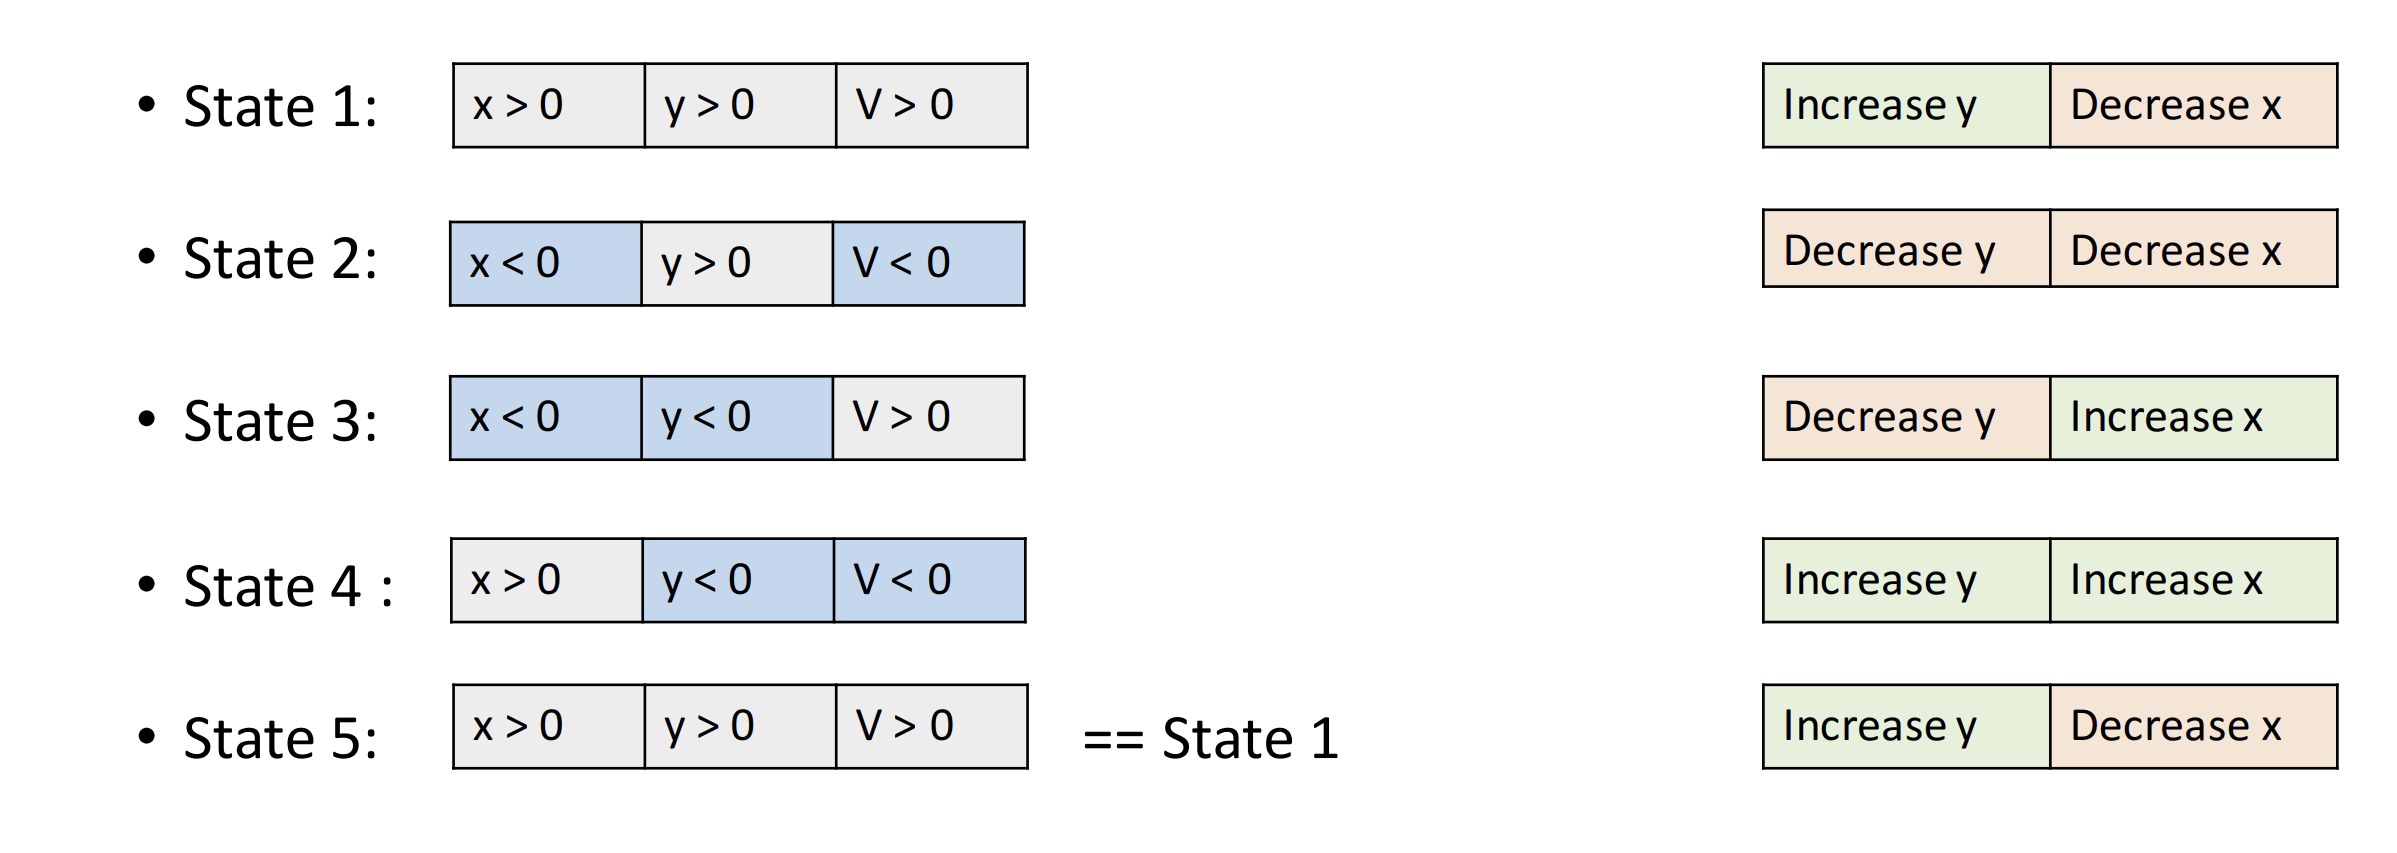
\includegraphics{plots/nonconverge.png}}
      %\tiny{\\Credit: https://slazebni.cs.illinois.edu/spring17/lec11_gan.pdf}
%   \end{figure}

%\end{frame}

%-------------------
%\begin{frame} {Adversarial Training}
%\begin{itemize}
%\vspace{12mm}
%\item So, GANs have intuitive appeal and produce state-of-the-art results but the reason they are such an important breakthrough is that they introduce a whole new paradigm to training deep neural networks: Adversarial Training$^1$.
%\vspace{4mm}
%\item Compared to plain-vanilla gradient descent, 
%adversarial training is a whole different beast; one that we have not figured out how to tame (yet).
%\vspace{4mm}
%\item To illustrate this, let us look at a simple example.
%\vspace{6mm}
%\end{itemize}
%\tiny{1. The term 'adversarial training' is used in slightly different contexts in the community. }
%\end{frame}

\begin{frame} {Adversarial Training -Example}
\begin{figure}
\centering
\scalebox{0.9}{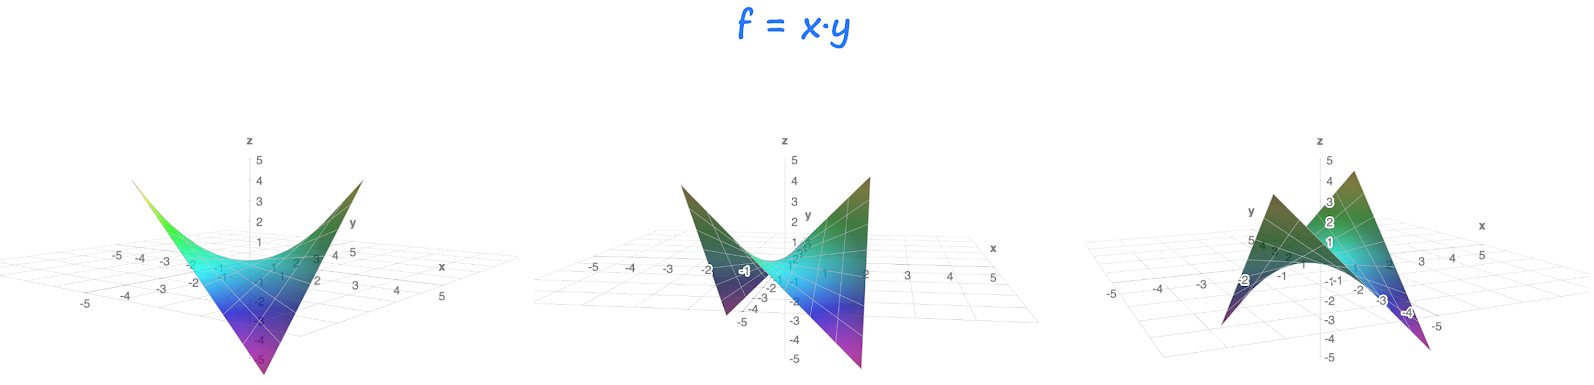
\includegraphics{plots/adv_xy.png}}
\end{figure}
\begin{itemize}
\item Consider the function $f(x,y) = xy$, where $x$ and $y$ are both scalars.
\item Player A can control $x$ and Player B can control $y$.
    \item The loss:
    \begin{itemize}
\item Player A: $L_{A}(x,y) = xy$
    \item Player B: $L_{B}(x,y) = -xy$
    \end{itemize}
\item This can be rewritten as $L(x,y) = \min \limits_x \max \limits_y xy$
    \item What we have here is a simple zero-sum game with its characteristic minimax loss.
\end{itemize}
\end{frame}

    
\begin{frame} {Possible behaviour \#1: Convergence}
  \begin{figure}
    \centering
     {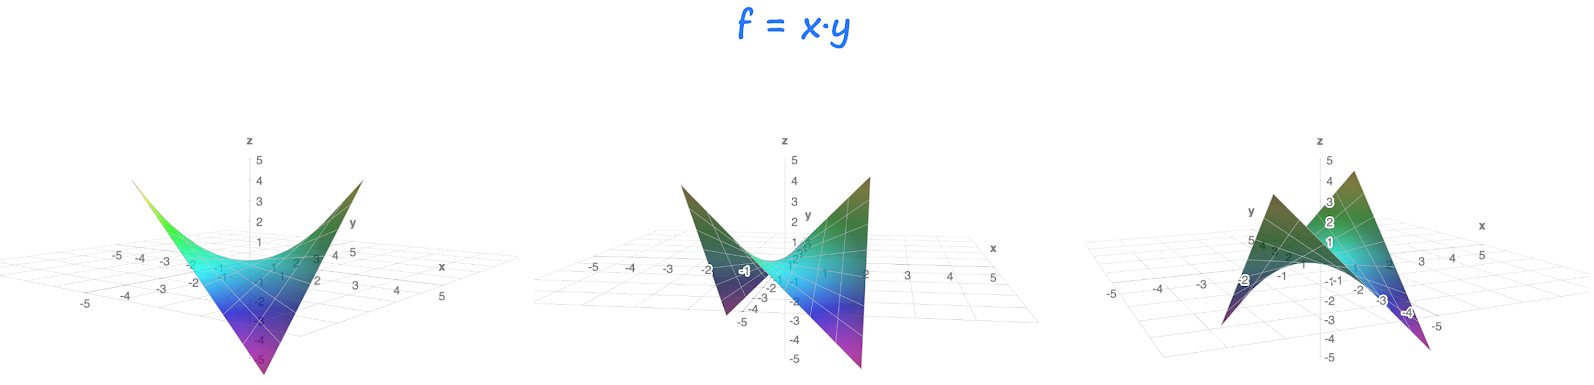
\includegraphics{plots/adv_xy.png}}
  \end{figure}
  \begin{itemize}
    \item The partial derivatives of the losses are:
     \begin{equation*}
       \frac {\partial{L_{A}}}{\partial x} = y \text{ , }
       \frac {\partial{L_{B}}}{\partial y} = -x
     \end{equation*}
    \item In adversarial training, both players perform gradient descent on their respective losses.
    \item %To perform simultaneous gradient descent, 
    We update $x$ with $x - \alpha \cdot y$ and $y$ with $y + \alpha \cdot x$ simultaneously in one iteration, where $\alpha$ is the learning rate.
  \end{itemize}
\end{frame}

\begin{frame} {Possible behaviour \#1: Convergence}
  \begin{figure}
    \centering
      \scalebox{0.9}{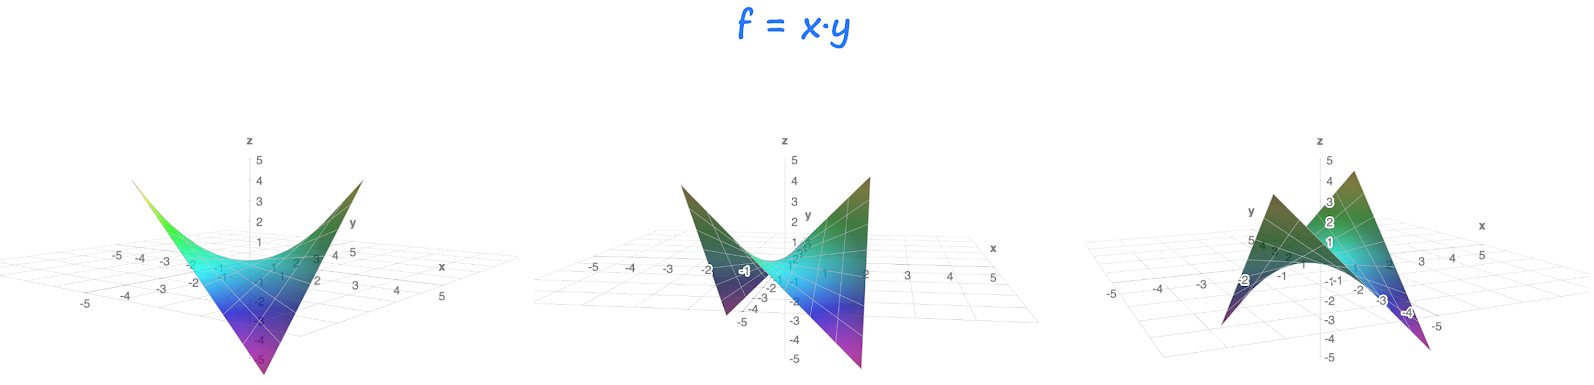
\includegraphics{plots/adv_xy.png}}
  \end{figure}
  \begin{itemize}
    \item In order for simultaneous gradient descent to converge to a fixed point, both gradients have to be simultaneously 0.
    \item They are both (simultaneously) zero only for the point (0,0).
    \item This is a saddle point of the function $f(x,y) = xy$.
    \begin{itemize}
       \item The fixed point for a minimax game is typically a saddle point.
      \item Such a fixed point is an example of a Nash equilibrium.
    \end{itemize}
    \item In adversarial training, convergence to a fixed point is \textbf{not} guaranteed.
  \end{itemize}
\end{frame}

\begin{frame} {Possible behaviour \#2: Chaotic behaviour}
  \begin{figure}
    \centering
      \scalebox{0.6}{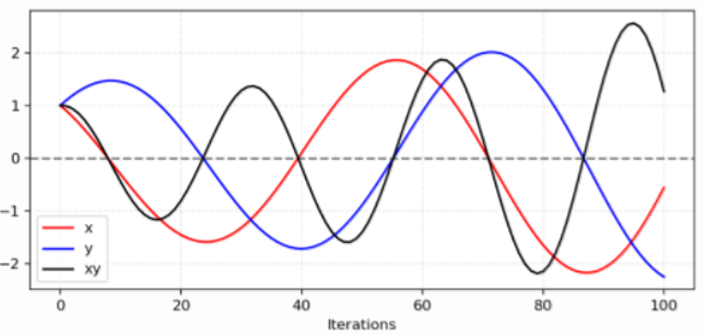
\includegraphics{plots/sim_grad.png}}
      \tiny{\\Credit: Lilian Weng}
      \caption{\footnotesize A simulation of our example for updating x to minimize xy and updating y to minimize -xy. The learning rate $\alpha$ = 0.1. With more iterations, the oscillation grows more and more unstable.}
  \end{figure}
  \begin{itemize}
    \item Once $x$ and $y$ have different signs, every following gradient update causes huge oscillation and the instability gets worse in time, as shown in the figure.
  \end{itemize}
\end{frame}


\begin{frame} {Possible behaviour \#3: Cycles}
  \begin{figure}
    \centering
      \scalebox{0.3}{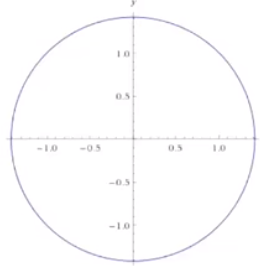
\includegraphics{plots/adv_cycle.png}}
      \tiny{\\Credit: Goodfellow}
      \caption{\footnotesize Simultaneous gradient descent with an infinitesimal step size can result in a circular orbit in the parameter space.}
  \end{figure}
  \begin{itemize}
    \item A discrete example: A never-ending game of Rock-Paper-Scissors where player A chooses 'Rock' $\rightarrow$ player B chooses 'Paper' $\rightarrow$ A chooses 'Scissors' $\rightarrow$ B chooses 'Rock' $\rightarrow$ ...
   % \item In GAN training, this happens when the generator keeps switching the category of the samples generated without a noticeable improvement in image quality for any category.
   \item  \textbf{Takeaway:} Adversarial training is highly unpredictable. It can get stuck in cycles or become chaotic.
  \end{itemize}
\end{frame}


\begin{frame} {Non-stationary loss surface}
   \begin{itemize}
     \item %Once again, it is extremely important to note that 
     From the perspective of one of the players, the loss surface changes every time the other player makes a move.
  \vspace{2mm}
     \item This is in stark contrast to  (full batch) gradient descent where the loss surface is stationary no matter how many iterations of gradient descent are performed.
%  \vspace{2mm}
   %  \item It's \textit{somewhat} analogous to a game of football played by two players where the goalposts for a given player changes position every time the opponent kicks the ball and vice versa!
%   \vspace{2mm}
 %   \item The only way this game ends(\textit{if} it ends, that is) is if the ball goes through both players' goalposts simultaneously.
%   \vspace{2mm}
%    \item This is what a saddle point represents. It is simultaneously a minimum for the first player and a maximum for the second player.

   \end{itemize}
 \end{frame}

\begin{frame} {Illustration of Convergence}
  \begin{figure}
    \centering
      \scalebox{0.8}{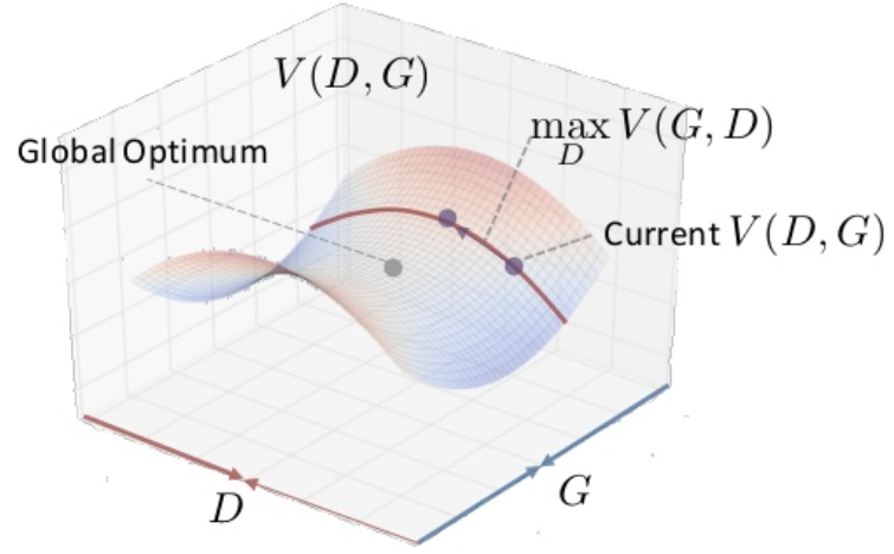
\includegraphics{plots/illus_conv_one.png}}
      \tiny{\\Credit: Mark Chang}
  \end{figure}
\end{frame}

\begin{frame} {Illustration of Convergence: Final Step}
  \begin{figure}
    \centering
      \scalebox{0.8}{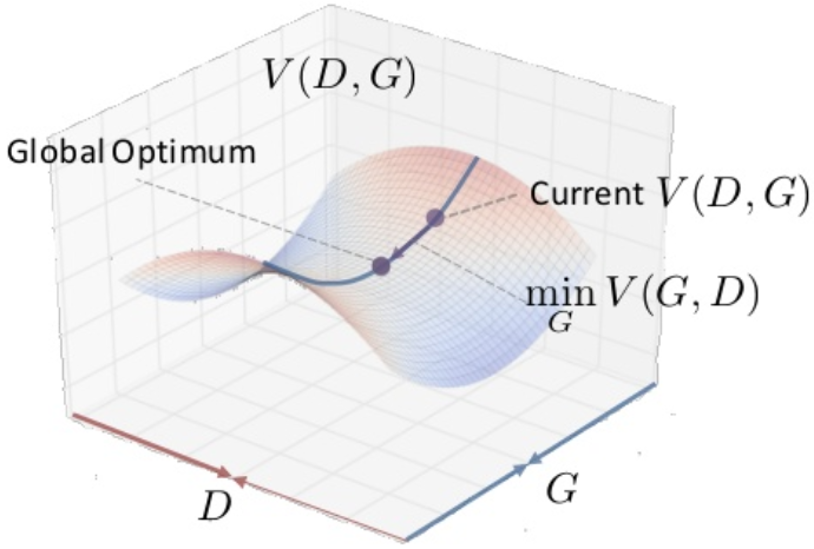
\includegraphics{plots/illus_conv_two.png}}
      \tiny{\\Credit: Mark Chang}
  \end{figure}
  Such convergence is not guaranteed, however.
\end{frame}

%\begin{frame} {Toy Example: Estimating a 1D Gaussian}
%  \vspace{10mm}
%  \begin{itemize}
%    \item Our target distribution is a simple Gaussian with mean 4 and standard deviation of 0.5.
%    \begin{figure}
%    \centering
%      \scalebox{0.66}{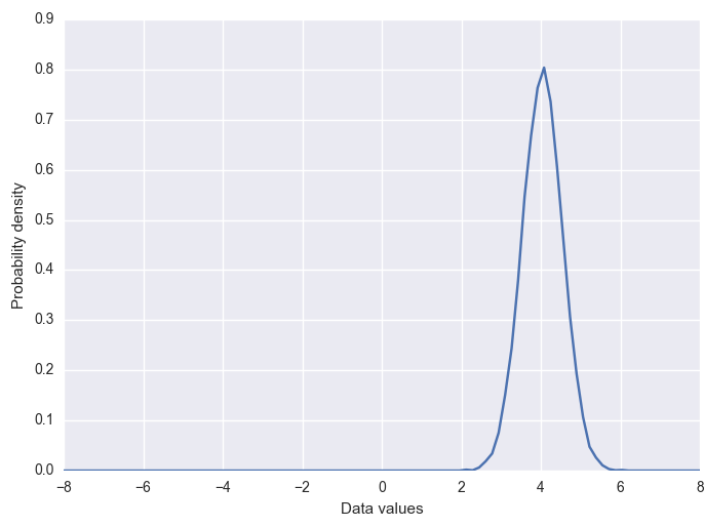
\includegraphics{plots/toy_gaussian.png}}
%      \tiny{\\Source: Aylien}
%  \end{figure}
%  \end{itemize}
%\end{frame}
%
%\begin{frame} {Toy Example: Estimating a 1D Gaussian}
%  \begin{itemize}
%    \item Our generator
%      \begin{itemize}
%        \item Takes a scalar noise input
%        \item Has only a single hidden layer with a softplus activation
%        \item The output layer has only a single neuron with a linear activation
%      \end{itemize}
%  \vspace{4mm}
%    \item Our discriminator
%      \begin{itemize}
%        \item Has 3 hidden layers with 'tanh' activations
%        \item The output layer once again has a single neuron with a sigmoid activation
%      \end{itemize}
%  \vspace{4mm}
%    \item Loss: Non-saturating Loss
%  \vspace{4mm}
%    \item Optimizer: Gradient Descent with exponential learning rate decay
%  \end{itemize}
%\end{frame}
%
%\begin{frame} {Toy Example: Estimating a 1D Gaussian}
%
%  \begin{itemize}
%  \item After training, the the two distributions look like this:
%  \begin{figure}
%    \centering
%      \scalebox{0.75}{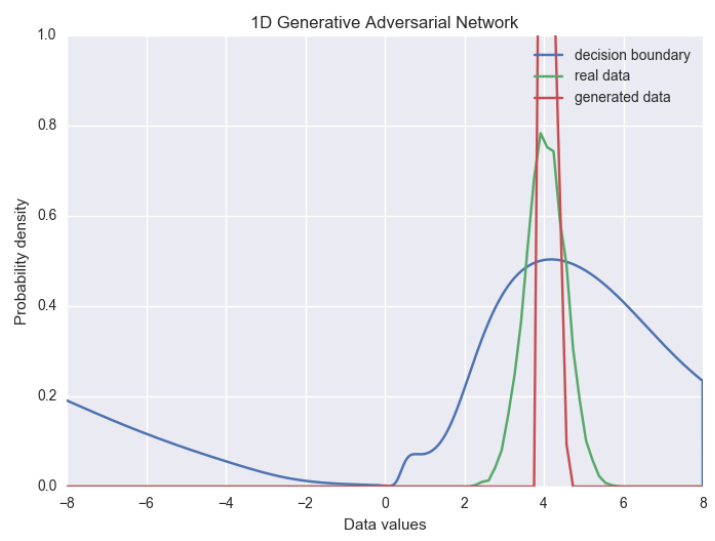
\includegraphics{plots/gan_gaussian_post.png}}
%      \tiny{\\Source: Aylien}
%  \end{figure}
%  \item This makes sense intuitively.If the generator just produces the mean value of the real data in this simple example, then it is going to be quite likely to fool the discriminator.
%  \end{itemize}
%\end{frame}

\begin{frame} {Challenges for GAN Training}

  \begin{itemize}
    \item Non-convergence: the model parameters oscillate, destabilize and never converge.
    \item Mode collapse: the generator collapses which produces limited varieties of samples.
     \item Diminished gradient: the discriminator gets too successful that the generator gradient vanishes and learns nothing.
     \item Unbalance between the generator and discriminator causing overfitting.
     \item Highly sensitive to the hyperparameter selections.
  \end{itemize}
\end{frame}


%\begin{frame} {Mode collapse}
%\vspace{2mm}
%Real-life data distributions are multimodal. For example, in MNIST, there are 10 major modes from digit '0' to digit '9'. The samples below are generated by two different GANs. The top row produces all 10 modes while the second row creates a single mode only (the digit '6'). This problem is called mode collapse when only a few modes of data are generated. 
%\vspace{2mm}
%  \begin{figure}
%    \centering
%      \scalebox{1}{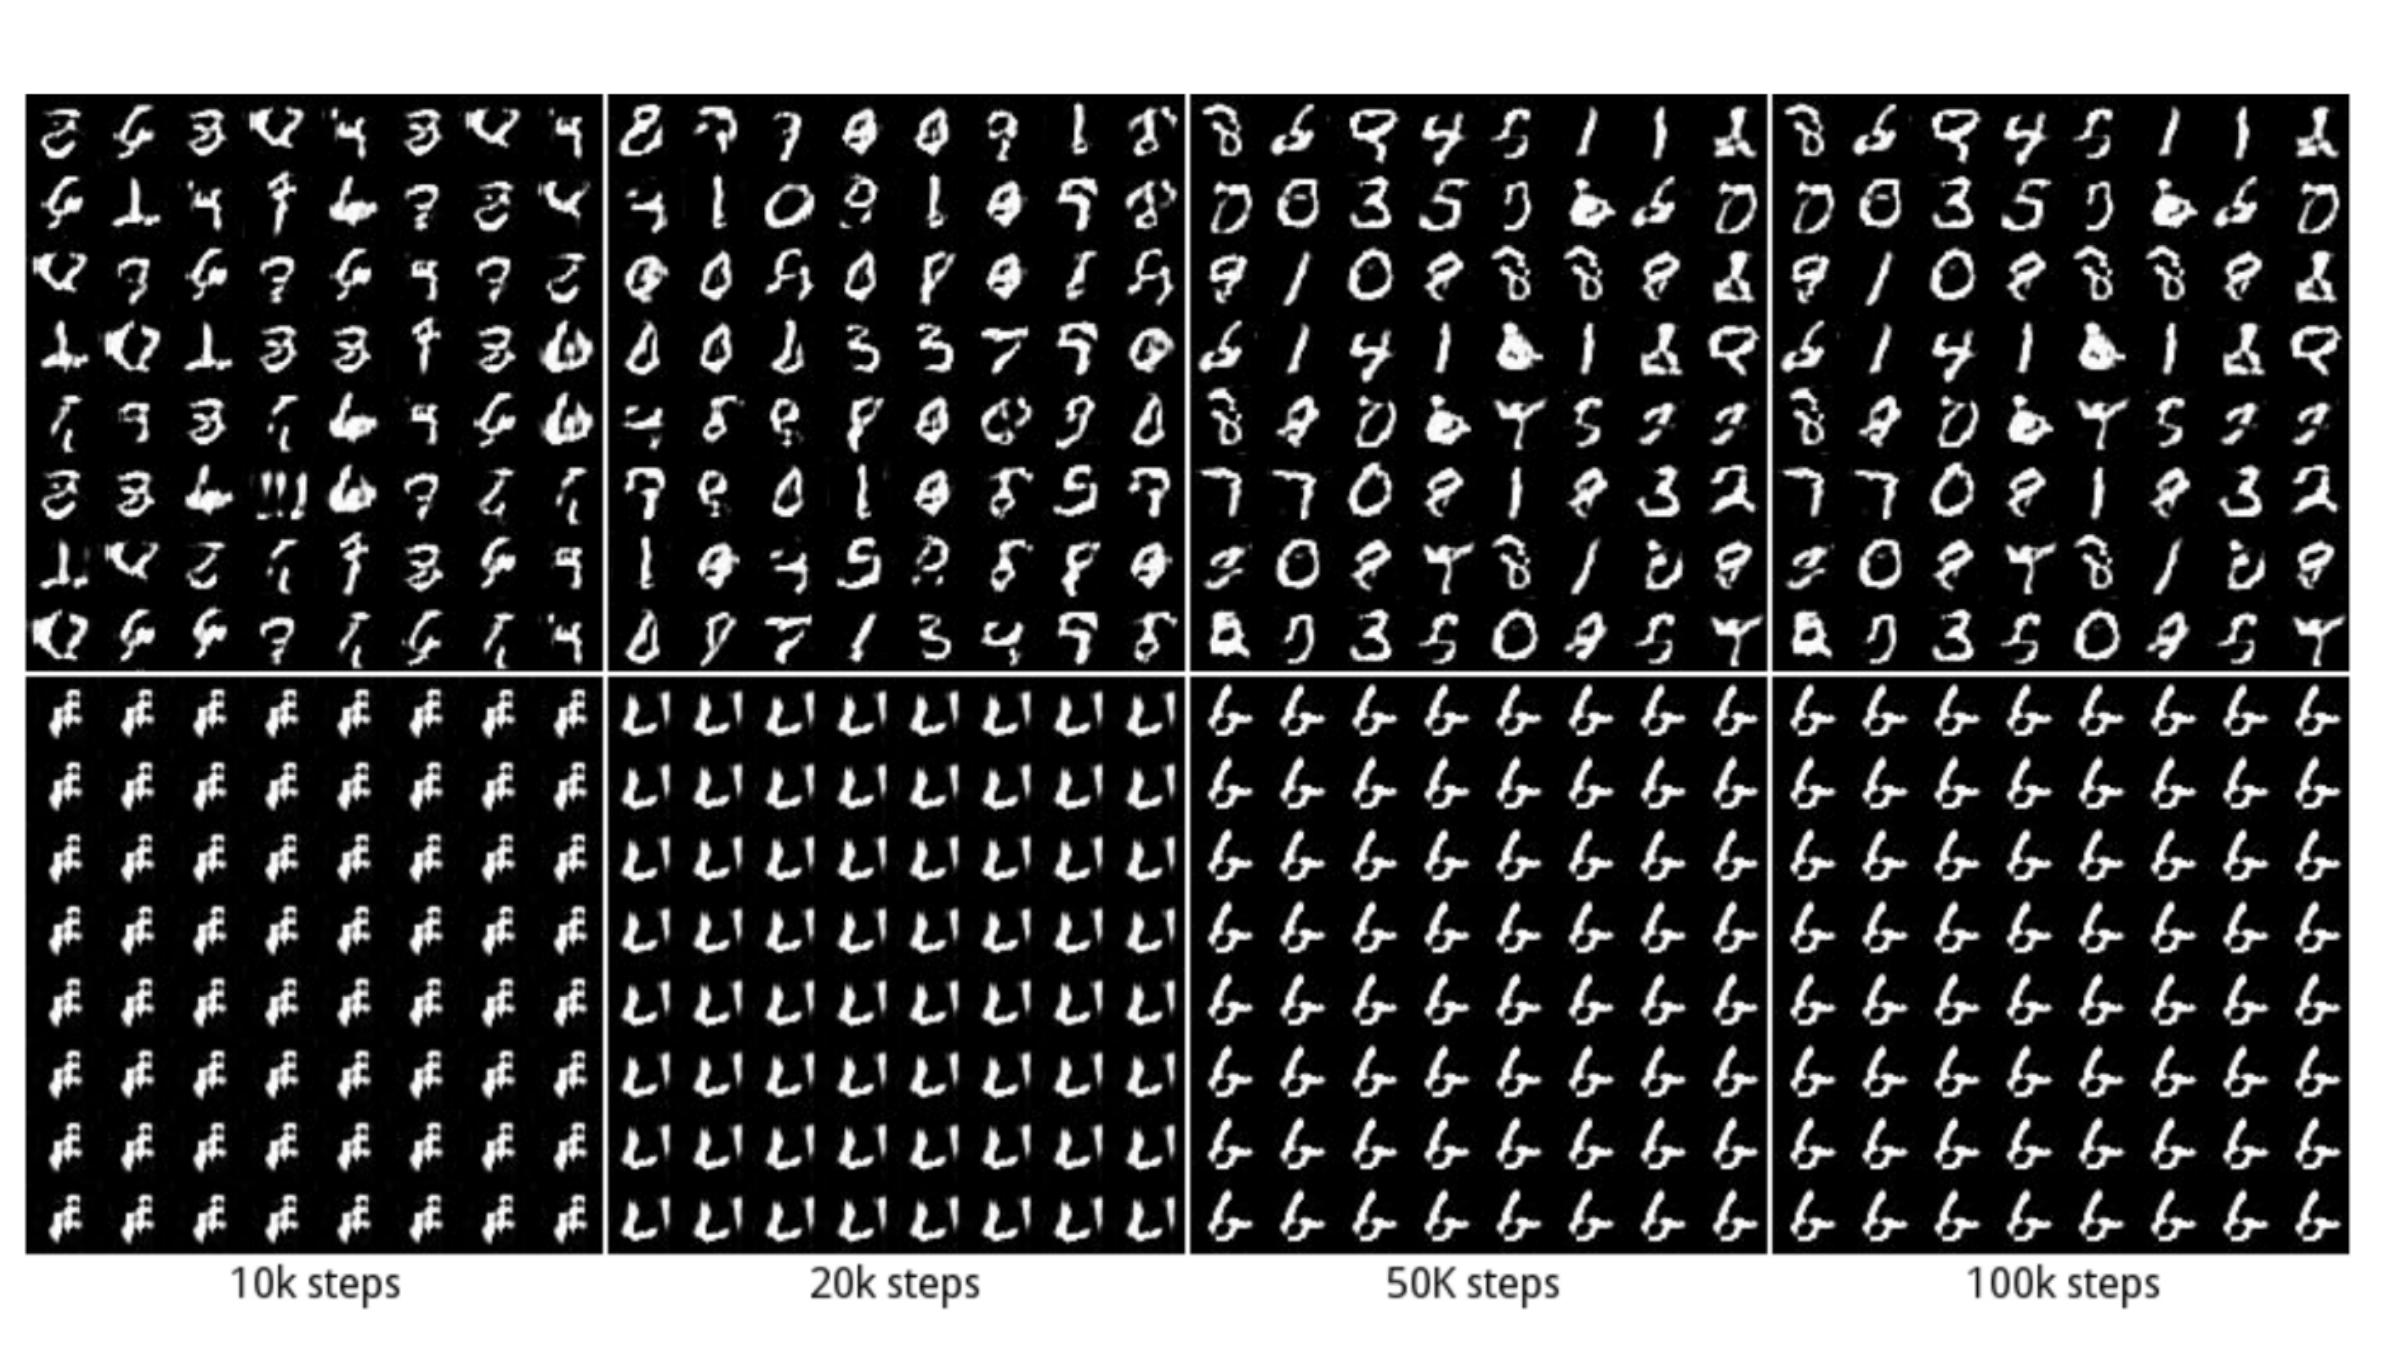
\includegraphics[width=7cm]{plots/modecollapse_mnist.png}}
%      \tiny{\\Credit: Luke Metz et al.(2017)}
%  \end{figure}
%\end{frame}

%\begin{frame} {Mode collapse- Example}
%\vspace{2mm}
%Generator fails to output diverse samples on Toy dataset
%\vspace{2mm}
%  \begin{figure}
%    \centering
%      \scalebox{1}{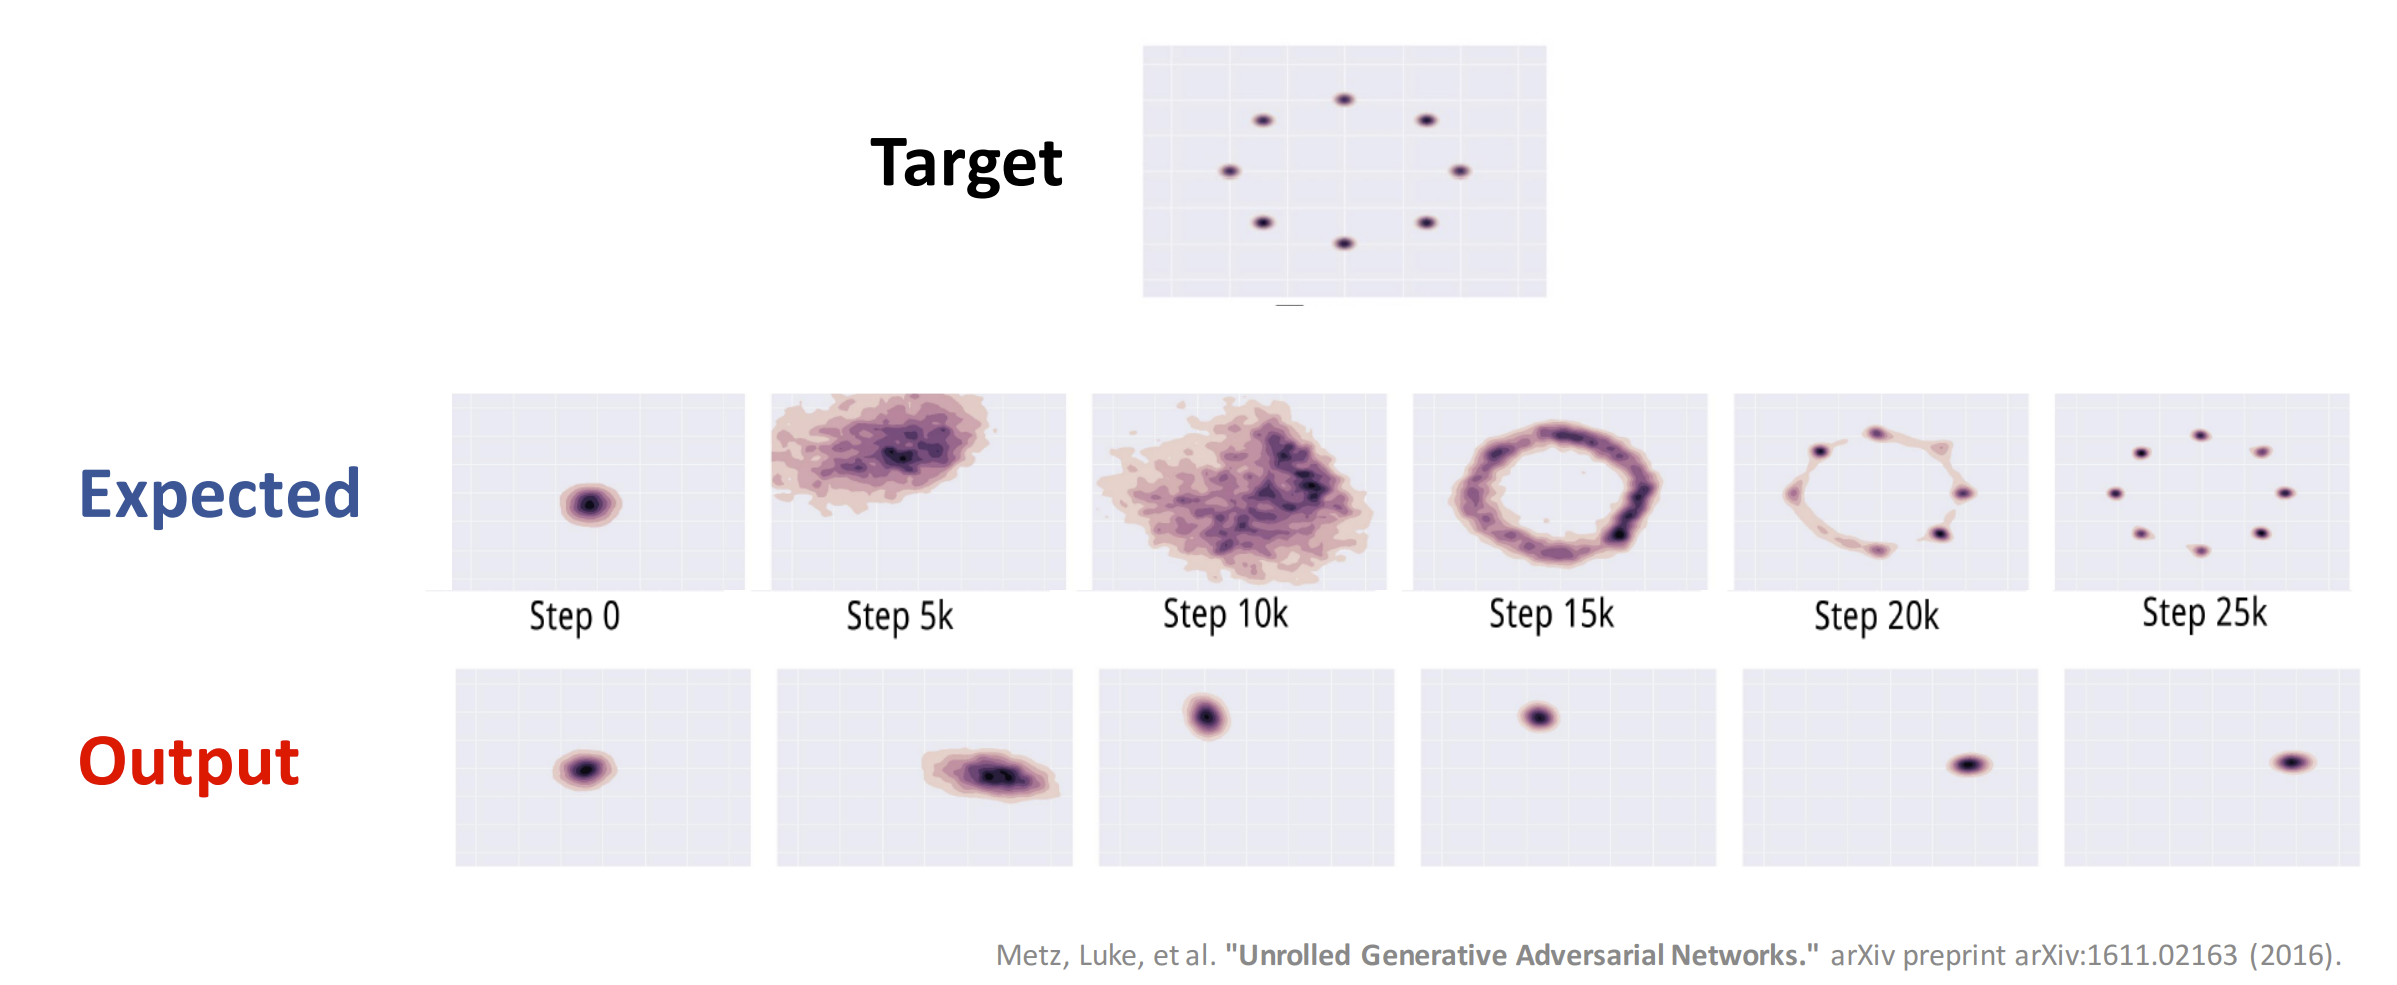
\includegraphics[width=12cm]{plots/toy.png}}
%  \end{figure}
%\end{frame}
%
%
%\begin{frame} {Solutions to tackle Mode Collapse}
%\vspace{2mm}
%  \begin{itemize}
%    \item Mini-batch GAN:
%      \begin{itemize}
%        \item Problem: Generator produces good samples but a very few of them, therefore discriminator can not tag them as fake!
%        \item Solution: Let the discriminator look at the entire batch instead of single example, If there is lack of diversity mark them fake! 
%        \item Result: Generator will be force to produce diverse samples!
%      \end{itemize}
%    \item Train with labels
%          \begin{itemize}
%            \item Label information of real data might help
%            \item Here, we train D with all categories instead of binary label!
%          \end{itemize}
%  \end{itemize}
%\end{frame}

%\begin{frame} {Vanishing gradients in JS-Divergence}
%\vspace{2mm}
%  \begin{itemize}
%    \item Recall that when the discriminator is optimal, the objective function for the generator is:\\
%     $\min \limits_G V(D^*,G) = 2 D_{JS} (p_r || p_g) - 2 \log 2 $
%    \vspace{2mm}
%    \item  The problem happens when the data distribution $q$ of the generator's images does not match with the ground truth $p$ for the real images.
%    \item  Let's consider q with different means to study the gradient of $JS(p, q)$
%  \end{itemize}
%  
%    \begin{figure}
%    \centering
%      \scalebox{1}{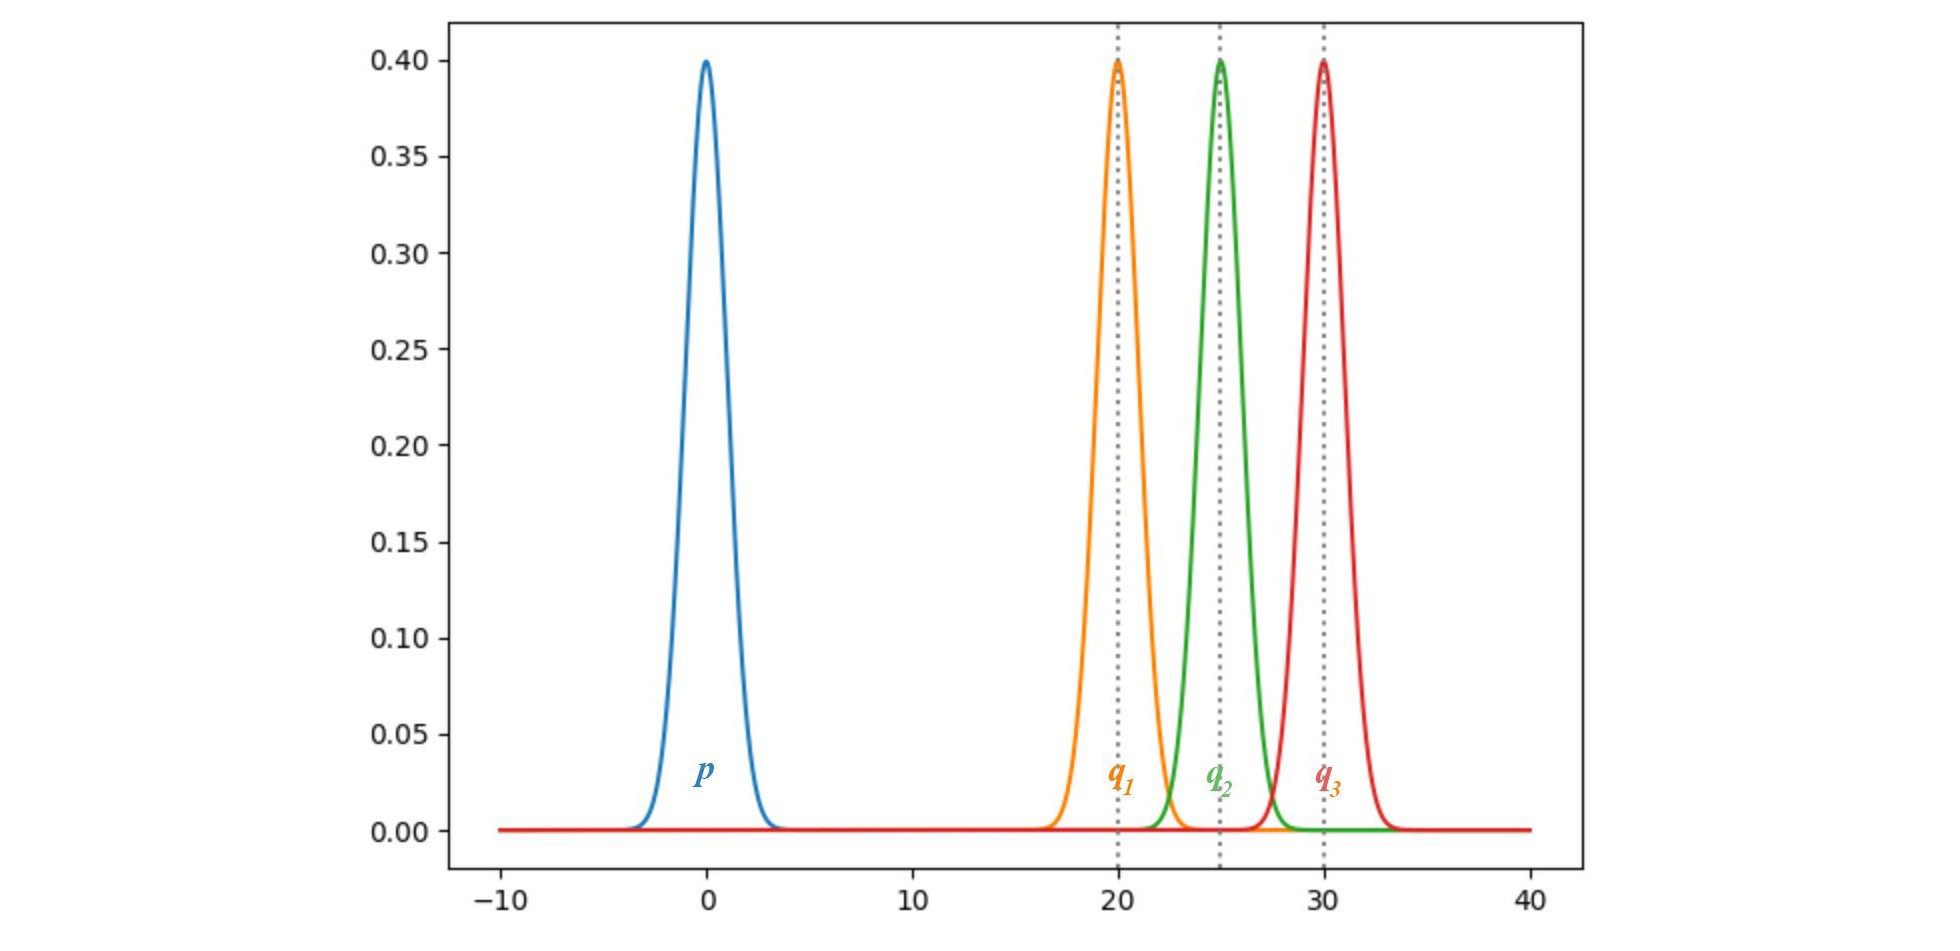
\includegraphics[width=7cm]{plots/JS1.jpeg}}
%      \tiny{\\Credit: Jonathan Hui.(2017)}
%  \end{figure}
%
%\end{frame}

%\begin{frame} {Vanishing gradients in JS-Divergence}
%    \vspace{2mm}
%    \begin{itemize}
%        \item Here, we plot the JS-divergence $JS(p, q)$ between $p$ and $q$ with means of $q$ ranging from 0 to 30. 
%\item As shown below, the gradient for the JS-divergence vanishes from $q_1$ to $q_3$.\\
%\item Results: The GAN generator will learn extremely slow to nothing when the cost is saturated in those regions. In early training, p and q are very different and the generator learns very slow.
%  \end{itemize}
%
%    \begin{figure}
%    \centering
%      \scalebox{1}{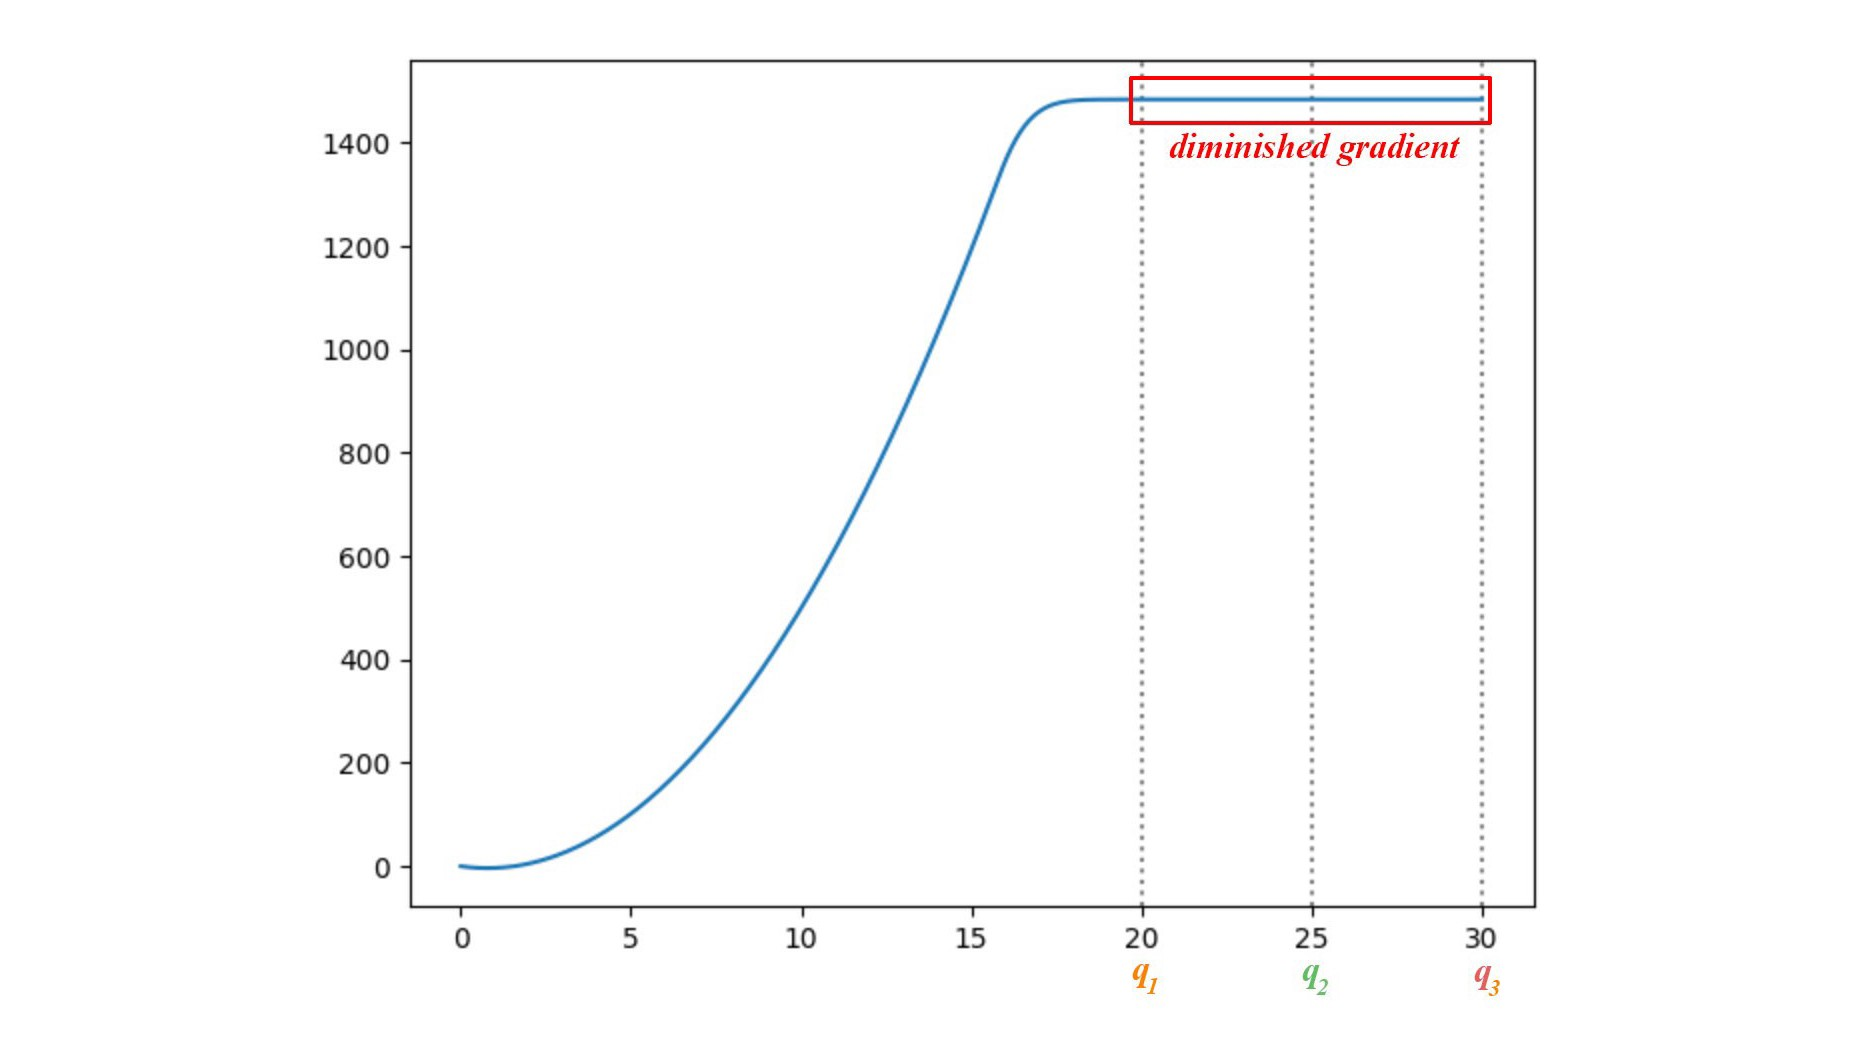
\includegraphics[width=7cm]{plots/JS2.jpeg}}
%      \tiny{\\Credit: Jonathan Hui.(2017)}
%  \end{figure}
%
%\end{frame}
%



%\begin{frame} {Trade-offs made by some common divergences}
%  \begin{figure}
%    \centering
%      \scalebox{1}{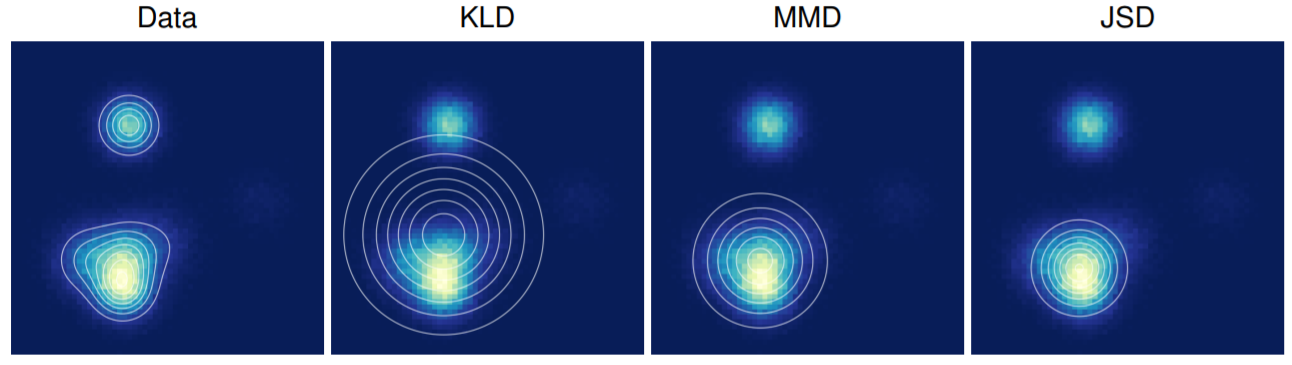
\includegraphics{plots/div_tradeoffs.png}}
%      \tiny{\\Source: Theis et al. 2016}
%      \caption{\small: An isotropic Gaussian distribution was fit to data drawn from a mixture of Gaussians by either minimizing Kullback-Leibler divergence (KLD), maximum mean discrepancy (MMD), or Jensen-Shannon divergence (JSD). The different fits demonstrate different tradeoffs made by the three measures of distance between distributions.}
% \end{figure}
%\end{frame}


%\begin{frame} {Trade-offs made by some common divergences}
%
%  \begin{figure}
%    \centering
%      \scalebox{0.8}{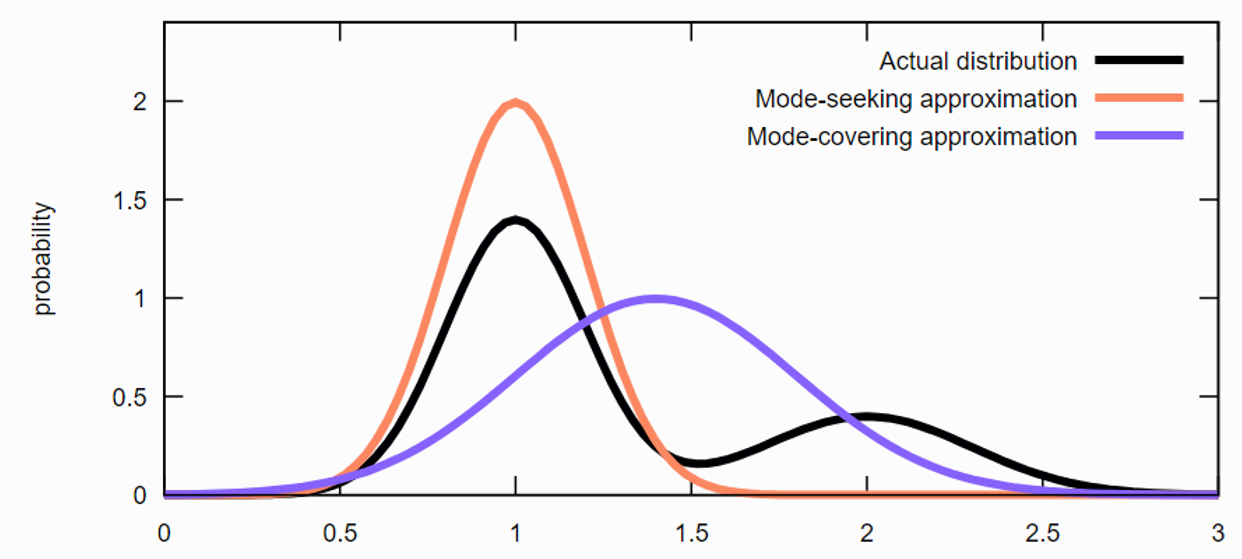
\includegraphics{plots/implicit_div.png}}
%      \tiny{\\Credit: Aiden NIbali}
%  \end{figure}
%  \begin{itemize}
%    \item In this simplified 1-dimensional example, $p_{\text{data}}(x)$ is a bimodal distribution, but $p_{\theta}(x)$ only has the modelling capacity of a single Gaussian.
%    \vspace{2mm}
%    \item Therefore, based on the divergence measure, $p_{\theta}(x)$ can either fit a single mode really well, i.e.~be `mode-seeking' (e.g.~JSD), or attempt to cover both modes, i.e. be `mode-covering' (e.g.~KLD).
%  \end{itemize}
%\end{frame}
%
%
%\begin{frame} {Alternative Divergences}
%
%Many common divergences, such as KL-divergence, Hellinger distance, and total variation distance, are special cases of f-divergence, coinciding with a particular choice of f. The following table lists many of the common divergences between probability distributions and the f function.
%
%  \begin{figure}
%    \centering
%      \scalebox{0.9}{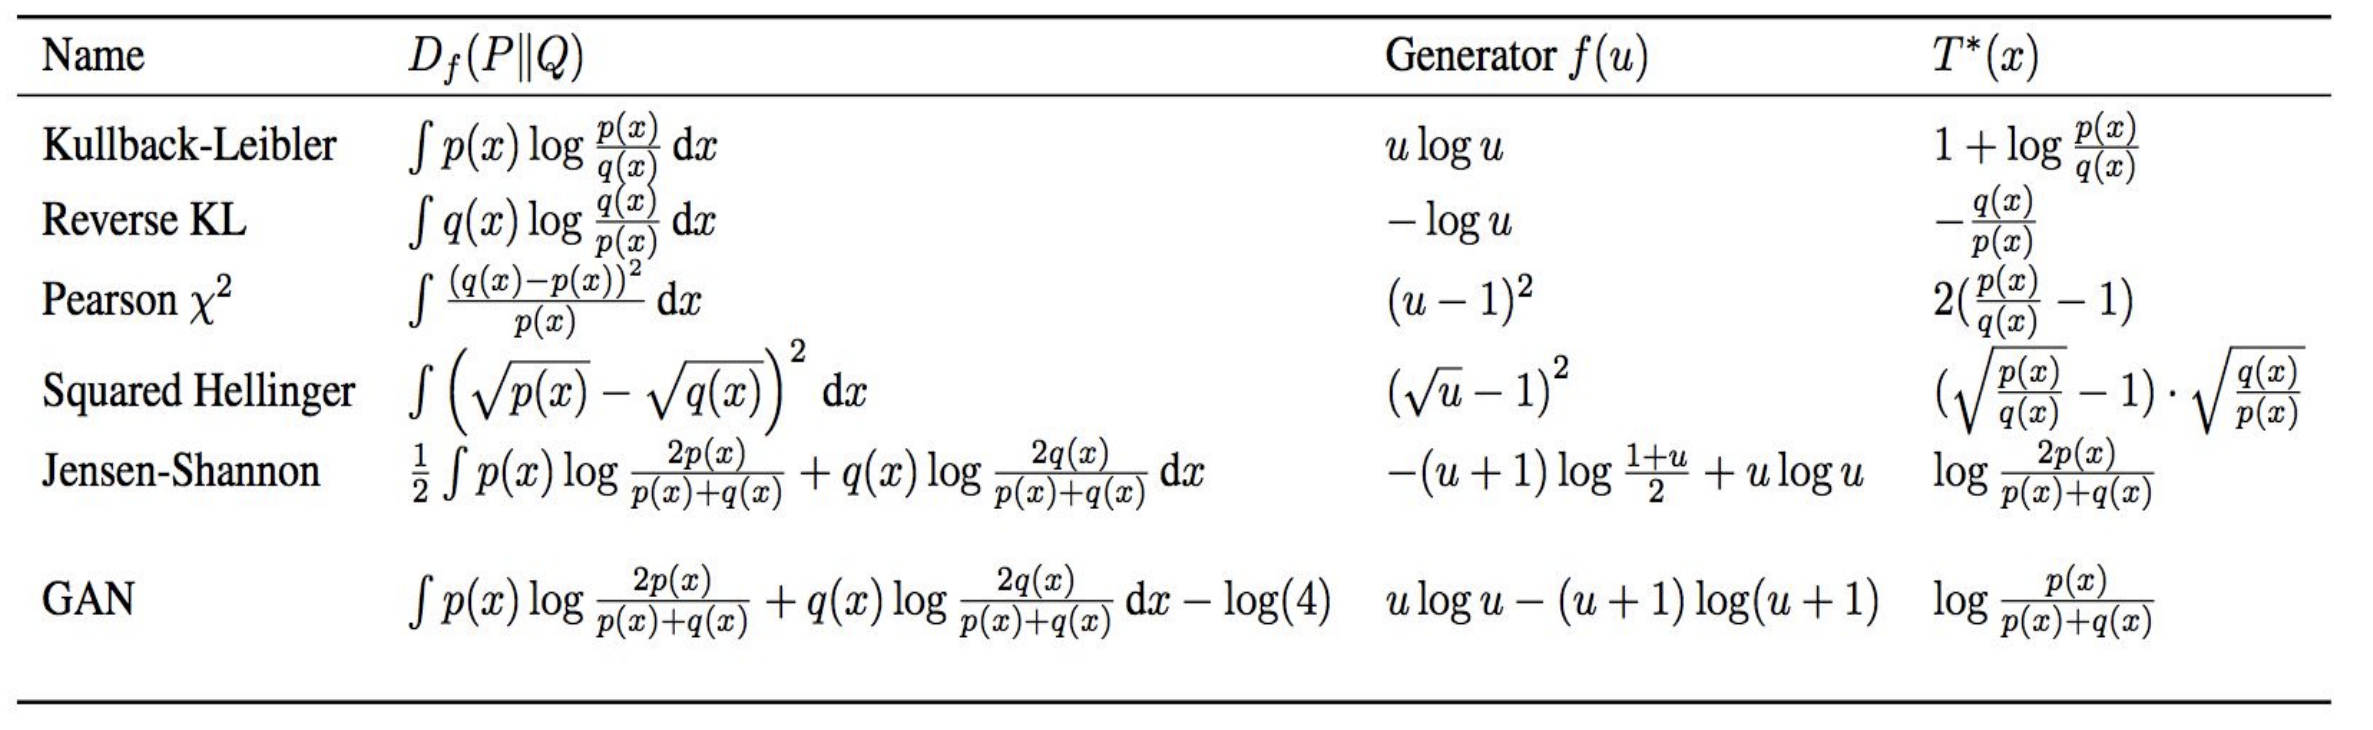
\includegraphics{plots/alternative_div.png}}
%      \tiny{\\Credit: Aiden NIbali}
%  \end{figure}
%  \begin{itemize}
%    \item We train a distribution $Q$ and an approximate the divergence with $T^{*}(x)$
%  \end{itemize}
%\end{frame}

%%%%-------------------------------------


%%%%%%%%%%%%%%%%%%%%%%%%%%%%%%%%%%%%%%%%%%%%%%%%%%%%%%%%%%%%%%%%%%
%%%%%%%%%%%%%%%%%%          REFERENCES          %%%%%%%%%%%%%%%%%%
%%%%%%%%%%%%%%%%%%%%%%%%%%%%%%%%%%%%%%%%%%%%%%%%%%%%%%%%%%%%%%%%%%
\begin{vbframe}
\frametitle{References}
\footnotesize{
\begin{thebibliography}{99}
% %%%%%%%%%%%%%%%%%%%%%%%%%%%%%%%%%%
% \bibitem[Zhang et al., 2017]{1} Han Zhang, Tao Xu, Hongsheng Li, Shaoting Zhang, Xiaogang Wang, Xiaolei Huang, Dimitris Metaxas (2017)
% \newblock StackGAN: Text to Photo-realistic Image Synthesis with Stacked Generative Adversarial Networks
% \newblock \emph{\url{https://arxiv.org/abs/1612.03242}}
% %%%%%%%%%%%%%%%%%%%%%%%%%%%%%%%%%%
% %%%%%%%%%%%%%%%%%%%%%%%%%%%%%%%%%
% \bibitem[Wang et al., 2017]{2} Ting-Chun Wang, Ming-Yu Liu, Jun-Yan Zhu, Andrew Tao, Jan Kautz, Bryan Catanzaro (2017)
% \newblock High-Resolution Image Synthesis and Semantic Manipulation with Conditional GANs
% \newblock \emph{\url{https://arxiv.org/abs/1711.11585}}
% %%%%%%%%%%%%%%%%%%%%%%%%%%%%%%%%%%
%%%%%%%%%%%%%%%%%%%%%%%%%%%%%%%%%
%\bibitem[Goodfellow et al., 2014]{5} Ian J. Goodfellow, Jean Pouget-Abadie, Mehdi Mirza, Bing Xu, David Warde-Farley, Sherjil Ozair, Aaron Courville, Yoshua Bengio (2014)
%\newblock Generative Adversarial Networks
%\newblock \emph{\url{https://arxiv.org/abs/1406.2661}}
%%%%%%%%%%%%%%%%%%%%%%%%%%%%%%%%%%
%%%%%%%%%%%%%%%%%%%%%%%%%%%%%%%%%
%\bibitem[Pascual et al., 2017]{6} Santiago Pascual, Antonio Bonafonte, Joan Serra (2017)
%\newblock SEGAN: Speech Enhancement Generative Adversarial Network
%\newblock \emph{\url{https://arxiv.org/abs/1703.09452}}
%%%%%%%%%%%%%%%%%%%%%%%%%%%%%%%%%%
%%%%%%%%%%%%%%%%%%%%%%%%%%%%%%%%%
\bibitem[Goodfellow, 2016]{7} Ian Goodfellow (2016)
\newblock NIPS 2016 Tutorial: Generative Adversarial Networks
\newblock \emph{\url{https://arxiv.org/abs/1701.00160}}
%%%%%%%%%%%%%%%%%%%%%%%%%%%%%%%%%%
%%%%%%%%%%%%%%%%%%%%%%%%%%%%%%%%%
\bibitem[Weng, 2017]{8} Lilian Weng (2017)
\newblock From GAN to WGAN
\newblock \emph{\url{https://lilianweng.github.io/lil-log/2017/08/20/from-GAN-to-WGAN.html}}
%%%%%%%%%%%%%%%%%%%%%%%%%%%%%%%%%%
%%%%%%%%%%%%%%%%%%%%%%%%%%%%%%%%%
\bibitem[Chang, 2016]{9} Mark Chang (2016)
\newblock Generative Adversarial Networks
\newblock \emph{\url{https://www.slideshare.net/ckmarkohchang/generative-adversarial-networks}}
%%%%%%%%%%%%%%%%%%%%%%%%%%%%%%%%%%
%%%%%%%%%%%%%%%%%%%%%%%%%%%%%%%%%
%\bibitem[Theis et al., 2016]{10} Lucas Theis, Aaron van den Oord, Matthias Bethge (2016)
%\newblock A note on the evaluation of generative models
%\newblock \emph{\url{https://arxiv.org/abs/1511.01844}}
%%%%%%%%%%%%%%%%%%%%%%%%%%%%%%%%%%
%%%%%%%%%%%%%%%%%%%%%%%%%%%%%%%%%
%\bibitem[Nibali, 2016]{11} Aiden Nibali (2016)
%\newblock The GAN objective, from practice to theory and back again
%\newblock \emph{\url{https://aiden.nibali.org/blog/2016-12-21-gan-objective/}}
%%%%%%%%%%%%%%%%%%%%%%%%%%%%%%%%%%%
%%%%%%%%%%%%%%%%%%%%%%%%%%%%%%%%%
%\bibitem[Mirza, 2014]{12} Mehdi Mirza, Simon Osindero (2014)
%\newblock Conditional Generative Adversarial Nets
%\newblock \emph{\url{https://arxiv.org/abs/1411.1784}}
%%%%%%%%%%%%%%%%%%%%%%%%%%%%%%%%%%%
%%%%%%%%%%%%%%%%%%%%%%%%%%%%%%%%%%
%\bibitem[Isola et al., 2016]{13} Phillip Isola, Jun-Yan Zhu, Tinghui Zhou, Alexei A. Efros (2016)
%\newblock Image-to-Image Translation with Conditional Adversarial Networks
%\newblock \emph{\url{https://arxiv.org/abs/1611.07004}}
%%%%%%%%%%%%%%%%%%%%%%%%%%%%%%%%%%%
%%%%%%%%%%%%%%%%%%%%%%%%%%%%%%%%%%
%\bibitem[Perarnau, 2017]{14} Guim Perarnau (2017)
%\newblock Fantastic GANs and where to find them
%\newblock \emph{\url{https://guimperarnau.com/blog/2017/03/Fantastic-GANs-and-where-to-find-them}}
%%%%%%%%%%%%%%%%%%%%%%%%%%%%%%%%%%%
%%%%%%%%%%%%%%%%%%%%%%%%%%%%%%%%%


\end{thebibliography}
}
\end{vbframe}
%%%%%%%%%%%%%%%%%%%%%%%%%%%%%%%%%%%%%%%%%%%%%%%%%%%%%%%%%%%%%%%%%%
%%%%%%%%%%%%%%%%%%%%%%%%%%%%%%%%%%%%%%%%%%%%%%%%%%%%%%%%%%%%%%%%%%

\endlecture
\end{document}